\Class{Psychic Warrior}
{The body is not bound to the forms and function you were born with. To master the art of delivering death, you must break your given mold.}{Tharlkar, psychic sense}

The term ``psychic warrior'' is a loose translation of the thri-kreen word ``chakak,'' which is better translated as ``mind warrior.'' In the Tablelands, non-kreen psychic warriors have long been known as ``mercenary psionicists.''

\PsychicTable{The Psychic Warrior}{
1  & +0         & +2  & +0 & +2  & Bonus feat & 0   & 1  & 1st\\
2  & +1         & +3  & +0 & +3  & Bonus feat & 2   & 2  & 1st\\
3  & +2         & +3  & +1 & +3  &            & 4   & 3  & 1st\\
4  & +3         & +4  & +1 & +4  &            & 8   & 4  & 2nd\\
5  & +3         & +4  & +1 & +4  & Bonus feat & 12  & 5  & 2nd\\
6  & +4         & +5  & +2 & +5  &            & 18  & 6  & 2nd\\
7  & +5         & +5  & +2 & +5  &            & 24  & 7  & 3rd\\
8  & +6/+1      & +6  & +2 & +6  & Bonus feat & 32  & 8  & 3rd\\
9  & +6/+1      & +6  & +3 & +6  &            & 40  & 9  & 3rd\\
10 & +7/+2      & +7  & +3 & +7  &            & 50  & 10 & 4th\\
11 & +8/+3      & +7  & +3 & +7  & Bonus feat & 60  & 11 & 4th\\
12 & +9/+4      & +8  & +4 & +8  &            & 72  & 12 & 4th\\
13 & +9/+4      & +8  & +4 & +8  &            & 84  & 13 & 5th\\
14 & +10/+5     & +9  & +4 & +9  & Bonus feat & 98  & 14 & 5th\\
15 & +11/+6/+1  & +9  & +5 & +9  &            & 112 & 15 & 5th\\
16 & +12/+7/+2  & +10 & +5 & +10 &            & 128 & 16 & 6th\\
17 & +12/+7/+2  & +10 & +5 & +10 & Bonus feat & 144 & 17 & 6th\\
18 & +13/+8/+3  & +11 & +6 & +11 &            & 162 & 18 & 6th\\
19 & +14/+9/+4  & +11 & +6 & +11 &            & 180 & 19 & 6th\\
20 & +15/+10/+5 & +12 & +6 & +12 & Bonus feat & 200 & 20 & 6th\\
}

\subsection{Making a Psychic Warrior}
Despite his spectacular combat powers, a psychic warrior is not a typical front-line combatant. Although a fighter, barbarian, or gladiator might swing a sword more accurately, or with greater force, a psychic warrior depends on his repertoire of power and feats. A psychic warrior is the psionic equivalent of an eldritch knight or a warmage from other settings. A psychic warrior's role in the party isn't easily defined, but his combination of physical might, the Way, and martial arts is useful in almost any encounter.

\textbf{Races:} Practicing psionics as part of hunting or combat comes as naturally to a thri-kreen, as running comes to an elf. The Thri-kreen propensity to become ``chakak'' is rooted in the kreen ancestral memory. Becoming ``chakak'' is an almost unavoidable rite of kreen adulthood. Even kreen who focus their attentions in another class, such as the druid, tend to take at least one level as a psychic warrior. Nearly all pack-leaders and clutchleaders are accomplished chakak. Because of the clutch-mind, kreen chakak are far more cooperative, and infinitely less competitive with each other than the psychic warriors of other races.

Muls particularly excel as psychic warriors, as do humans, elves, and dwarves, to a lesser extent. Aarakocra and pterran psychic warriors are rare in those racial cultures, but individuals who take up the psychic warrior class tend to thrive. Halflings and jozhal psychic warriors are virtually unheard of.

\textbf{Alignment:} Psychic warriors tend towards neutrality with regards to good and evil, but they must be either lawful or chaotic. Chaotic psychic warriors, known commonly as ``mercenary psionicists,'' often work as attack thugs or assassins, though like bards, mercenary psionicists are notorious for switching allegiances according to the highest purse. Lawful psychic warriors, or ``mindguards,'' are the most sought-after personal guards for nobles and merchant lords. Like the elite rogue servants of the nobles, mindguards serve loyally in exchange for lavish compensation.

\subsection{Game Rule Information}

\textbf{Alignment:} Any lawful or chaotic.

\textbf{Hit Die:} d8.

\subsubsection{Class Skills}
\skill{Autohypnosis} (Wis), \skill{Climb} (Str), \skill{Concentration} (Con), \skill{Craft} (Int), \skill{Intimidate} (Cha), \skill{Jump} (Str), \skill{Knowledge} (psionics) (Int), \skill{Profession} (Wis), \skill{Ride} (Dex), and \skill{Search} (Int).

\textbf{Skill Points per Level:} 4 + Int modifier ($\times 4$ at 1st level).

\subsubsection{Class Features}

\textbf{Weapon and Armor Proficiency:} Psychic warriors are proficient with all simple and martial weapons, with all types of armor (heavy, medium, and light), and with shields (except tower shields).

\textbf{Power Points/Day:} A psychic warrior's ability to manifest powers is limited by the power points he has available. His base daily allotment of power points is given on \tabref{The Psychic Warrior}. In addition, he receives bonus power points per day if he has a high Wisdom score (see \tabref{Ability Scores and Bonus Power Points}). His race may also provide bonus power points per day, as may certain feats and items. A 1st-level psychic warrior gains no power points for his class level, but he gains bonus power points (if he is entitled to any), and can manifest the single power he knows with those power points.

\begin{figure*}[b!]
\centering
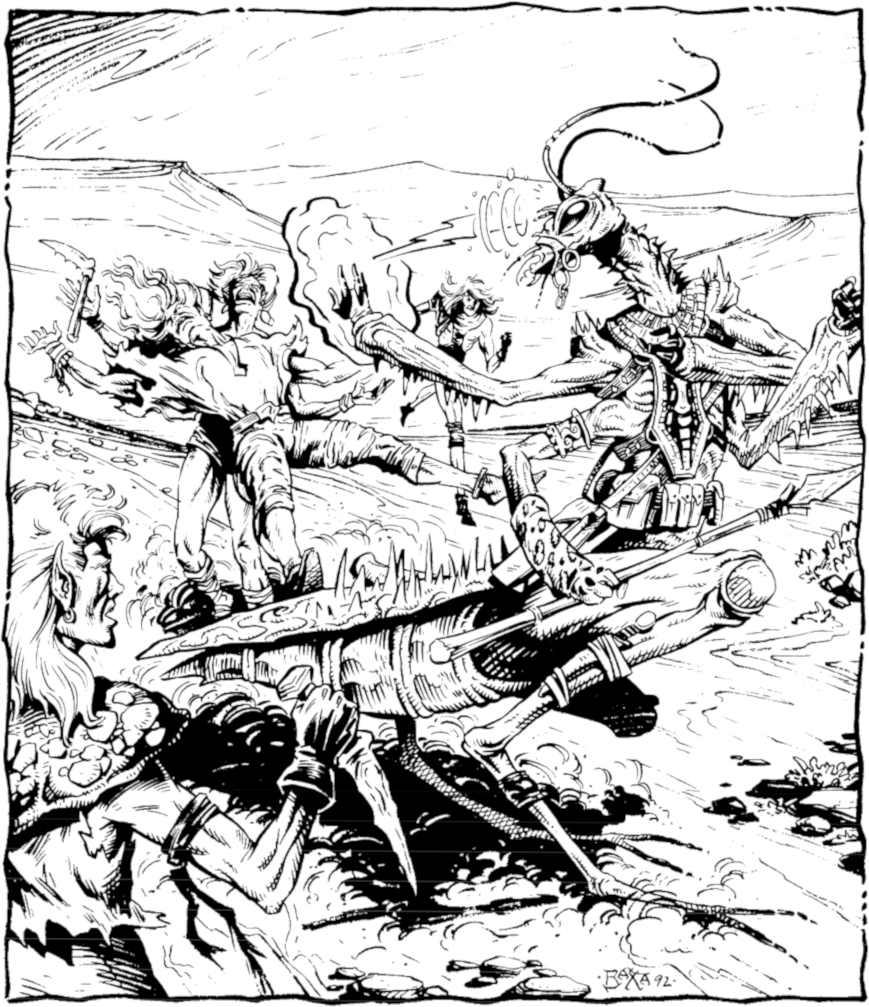
\includegraphics[width=\textwidth]{images/psywarrior-1.png}
\WOTC
\end{figure*}

\textbf{Powers Known:} A psychic warrior begins play knowing one psychic warrior power of your choice. Each time he achieves a new level, he unlocks the knowledge of a new power.

Choose the powers known from the psychic warrior power list. (Exception: The feat \feat{Expanded Knowledge} do allow a psychic warrior to learn powers from the lists of other classes.) A psychic warrior can manifest any power that has a power point cost equal to or lower than his manifester level.

The total number of powers a psychic warrior can manifest in a day is limited only by his daily power points.

A psychic warrior simply knows his powers; they are ingrained in his mind. He does not need to prepare them (in the way that some spellcasters prepare their spells), though he must get a good night's sleep each day to regain all his spent power points.

The Difficulty Class for saving throws against psychic warrior powers is 10 + the power's level + the psychic warrior's Wisdom modifier.

\textbf{Maximum Power Level Known:} A psychic warrior begins play with the ability to learn 1st-level powers. As he attains higher levels, he may gain the ability to master more complex powers.

To learn or manifest a power, a psychic warrior must have a Wisdom score of at least 10 + the power's level.

\textbf{Bonus Feats:} At 1st level, a psychic warrior gets a bonus combat-oriented feat in addition to the feat that any 1st level character gets and the bonus feat granted to a human character. The psychic warrior gains an additional bonus feat at 2nd level and every three levels thereafter (5th, 8th, 11th, 14th, 17th, and 20th). These bonus feats must be drawn from the feats noted as fighter bonus feats or psionic feats. The psychic warrior must still meet all prerequisites for the bonus feat, including ability score and base attack bonus minimums as well as class requirements. A psychic warrior cannot choose feats that specifically require levels in the fighter class unless he is a multiclass character with the requisite levels in the fighter class.

These bonus feats are in addition to the feats that a character of any class gains every three levels. A psychic warrior is not limited to fighter bonus feats and psionic feats when choosing these other feats.

\subsubsection{Ex-Psychic Warriors}
Any psychic warrior who ceases to be either lawful or chaotic, can no longer progress as a psychic warrior. She keeps all her powers known, power points, and bonus feats.

% \vskip2cm
\subsection{Playing a Psychic Warrior}
When you mold your body and mind with the same rigor as a dwarf tempers his steel, no feat or combat prowess is beyond you. Through it all, you seek to understand the secret knowledge of combat, and how to take your nexus---a point in the center of your being where physical, mental, and spiritual energy can be harnessed---to the next level. You know the exact extent of your abilities and how hard it was to achieve them, so you are prone to showing it off flamboyantly, and claim to fear nothing.

Psychic warriors adventure for a plethora of reasons. Neither the religious fervor of an elemental cleric nor the glory of the fighter causes you to travel the Tablelands. More than faith, more than glory, you seek martial perfection. Whether you find that perfection in the cannibal-filled jungles of the Forest Ridge, in the choking silt of the Silt Sea, or in the den of the deadly braxat, you are driven to learn it and master it.

% \begin{figure*}[b!]
% \centering
% 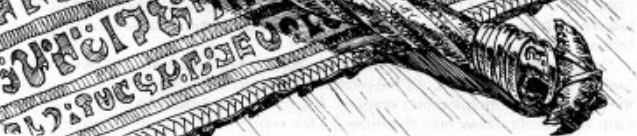
\includegraphics[width=\textwidth-2cm]{images/filler-2.png}
% \WOTC
% \end{figure*}

\subsubsection{Religion}
Religion might be entirely delusional to you, or you might find comfort in the elemental (or paraelemental) faiths, or even in the sorcerer-monarch of your city-state. If you are among the minority of psychic warriors who revere an element, you probably worship one associated with physical strength, such as Earth or Magma, or wisdom, such as Air or Sun.

\subsubsection{Other Classes}
Psychic warriors get along best with rogues, and to a lesser extent, fighters and bards. Generally, allies who show admiration for the psychic warriors' talents tend to get along well with the psychic warrior. Gladiators tend to get suspicious and envious of the psychic warrior's shows of unnatural and spectacular force, and many psychic warriors take a perverse pleasure in playing against the gladiator's jealousy, showing up the gladiator with spectacular stunts. Psychic warriors pretend to be indifferent to wizards, and to a lesser extent, psions, but many secretly envy the spectacle of a fireball.

\subsubsection{Combat}
You use your sword skills to defeat your foes as well as the limited access to manifest melee-oriented psionic powers. You have access to an amazing array of powerful combat feats. You have almost exclusive access to feats such as Deep Impact, Focused Sunder, and Wounding Attack, and you would do well to learn at least some of them. You have a limited selection of powers, so choose them carefully so you have a good mix of offensive, defensive and utility powers at your disposal.

\subsubsection{Advancement}
Your training began when you fought your way into an apprenticeship with a mentor---either a retired psychic warrior or an instructor in one of the many psionic academies dotting the Tablelands. You knew that finding that psychic warrior apprenticeship would not be that easy---that in fact, it would be an ordeal designed to test your body and mind to its fullest.

As a psychic warrior, your selection of psionic powers is paramount to your success. You might choose to focus on a specific psionic discipline, such as psychometabolism or psychokinesis, but learning a few powers from other disciplines is almost always advisable. True success in combat requires being ready for everything.

\vskip4cm
\subsection{Starting Packages}
\subsubsection{The Defender}
Mul Psychic Warrior

\textbf{Ability Scores:} Str 18, Dex 12, Con 15, Int 10, Wis 15, Cha 6.

\textbf{Skills:} \skill{Autohypnosis}, \skill{Concentration}, \skill{Intimidate}.

\textbf{Languages:} Common.

\textbf{Feat:} \feat{Combat Manifestation}.

\textbf{Weapons:} Great macahuitl (2d6/19--20)

Five javelins (1d6, 9 m).

\textbf{Armor:} Scale mail (+4 AC).

\textbf{Other Gear:} Standard adventurer's kit, 45 cp.

\vskip1cm
\subsubsection{The Destroyer}
Thri-kreen Psychic Warrior

\textbf{Ability Scores:} Str 17, Dex 17, Con 12, Int 8, Wis 16, Cha 4.

\textbf{Skills:} \skill{Concentration}, \skill{Intimidate}, \skill{Jump}.

\textbf{Languages:} Kreen.

\textbf{Feat:} \feat{Multiweapon Fighting}.

\textbf{Weapons:} Gythka (1d8/1d8)

Four chatkchas (1d6, 6 m).

\textbf{Armor:} Leather (+2 AC).

\textbf{Other Gear:} Standard adventurer's kit.

\vskip1cm
\subsubsection{The Skirmisher}
Human Psychic Warrior

\textbf{Ability Scores:} Str 14, Dex 13, Con 12, Int 10, Wis 15, Cha 8.

\textbf{Skills:} \skill{Concentration}, \skill{Intimidate}, \skill{Jump}, \skill{Psicraft}, \skill{Spot} (cc).

\textbf{Languages:} Common.

\textbf{Feat:} \feat{Dodge}, \feat{Weapon Focus} (glaive).

\textbf{Weapons:} Gouge (1d10/$\times$3)

Five javelins (1d6, 9 m).

\textbf{Armor:} Studded leather (+3 AC).

\textbf{Other Gear:} Standard adventurer's kit, 100 cp.

\subsection{Psychic Warriors on Athas}
\Quote{'Your studies have gone well, Turek,' he said quietly. 'You have learned the basics of psychic defense. It is time to practice your lessons.'

Turek nodded, his palms wet with sweat. He had known this was coming; he was one of the older students and it was time to begin his final studies before leaving the academy.

His master watched him without expression. Suddenly Turek found his attention ripped away from the patio and the master's physical form, being drawn inward. In his mind's eye a glowing sword appeared, poised to strike. 'I am the Sword', his master whispered. I pierce barriers and rend armor.' Turek swallowed nervously and summoned his defense. 'I am the Void, he thought over and over again. I cannot be found, I cannot be harmed.'

The Sword lunged forward, driving through the heart of the nothingness that cloaked Turek's presence...}{}

No place on Athas is safe from psionics. Armies and fortresses mean nothing to a master of the Way. To answer the threat of psionic attack, nobles and merchants retain the services of mercenary psionicists to guard against other users of the Way.

With a potential to advance in a number of different directions---offensive, defensive, support, and quick strike---psychic warriors make excellent additions to adventuring parties.

\subsubsection{Daily Life}

A psychic warrior spends the majority of his time perfecting his mind and body. The mental and spiritual demands of the Way require constant attention, so he can spare little time for carousing.

A psychic warrior with an apprentice spends much of his time training his student. A psychic warrior without one might or might not spend time seeking out one, according to his whims.

\subsubsection{Notables}

Hurgen Vurst, the half-giant garrison chief for Fort Harbeth is considered to be one of the most deadly specimens of his race, combining massive strength and a cleverness rarely found on half-giants. Chukaka the thri-kreen, was one of the first to be coin the term Kiltektet (the-learning-pack-who-enlightens), was a psychic warrior. Known as much for her wisdom, her teachings, as for her chatkchas, she is regarded by many the prototypical psychic warrior---serene, poised, and deadly.

\subsubsection{Organizations}

There is no specific organization that caters to psychic warriors. The Exalted Path (for males) and Serene Bliss (for females) orders in the city-state of Nibenay keep the city's ancient monastic tradition and they usually have several psychic warriors in their milieu. Villichi communities, female humans born with amazing psionic abilities, lie hidden in the deserts, harboring powerful psychic warriors.

\subsubsection{NPC Reactions}

As with fighters, individuals react to psychic warriors based on their previous interactions with other members of the class.

Gladiators have mixed feelings towards psychic warriors, they abilities can be of great value in the arena, but sometimes they feel a bit jealous of those abilities themselves, and they do not like other show offs competing for attention during gladiatorial matches. The only characters that psychic warriors as a rule will have an extremely hard time getting along with are other psychic warriors. Any party unfortunate enough to include more than one psychic warrior will be wrought with petty bickering, snide remarks, and endless competitions of spectacular force.

Merchants and nobles, on the other hand, greatly appreciate psychic warriors. They can always find ready employment as an elite mercenary, in the permanent guard of a noble family, or a merchant house sentry cadre.

\subsubsection{Psychic Warrior Lore}

Characters with ranks in \skill{Knowledge} (psionics) can research psychic warriors to learn more about them. When a character makes a skill check, read or paraphrase the following, including the information from lower DCs.

\textbf{DC 10:} A psychic warrior is a psionic sword-swinger who thinks he knows more about swordplay than anyone else.

\textbf{DC 15:} Like psions and wilders, psychic warrior walk the Unseen Way. Unlike them, psychic warriors train their bodies with the same rigor that they train their minds.

\textbf{DC 20:} Psychic warriors are strong, calm, and lethal. They gain the most psychic might of all those who study the Way.
